% IEEEtran two-column conference paper.
\documentclass[conference]{IEEEtran}

\usepackage{amsmath,amssymb,amsthm}
\usepackage{graphicx}
\usepackage{booktabs}
\usepackage{xcolor}
\usepackage[hidelinks]{hyperref}
\usepackage{subcaption}
\usepackage{cleveref}
\crefname{figure}{Fig.}{Figs.}
\Crefname{figure}{Fig.}{Figs.}
\crefname{table}{Table}{Tables}
\Crefname{table}{Table}{Tables}
\crefname{equation}{Eq.}{Eqs.}
\Crefname{equation}{Eq.}{Eqs.}
\crefname{section}{Sec.}{Secs.}
\Crefname{section}{Sec.}{Secs.}
\usepackage{cite}

\newtheorem{lemma}{Lemma}
\newtheorem{proposition}{Proposition}

\DeclareMathOperator*{\argmin}{arg\,min}
\newcommand{\R}{\mathbb{R}}
\newcommand{\opt}{^{\star}}
\newcommand{\hatp}[1]{\hat{#1}}

\begin{document}

\title{Differentiable Inverse DC-OPF: \\
Recovering Generator Costs and Capacities from Dispatch Data}

\author{\IEEEauthorblockN{Author}
\IEEEauthorblockA{EE364B, Stanford University \\
Spring 2025}}

\maketitle

\begin{abstract}
We study the inverse direct-current optimal power flow (DC-OPF) problem:
given a sequence of demand--dispatch pairs $\{(d_t,g_t)\}_{t=1}^T$ produced
by an unknown linear merit-order DC-OPF, recover the per-generator marginal
costs $f\opt$, generator capacities $g_{\max}\opt$, and line capacities
$p_{\max}\opt$. We pose this as a constrained convex regression problem and
solve it end-to-end by differentiating through a CVXPY-Layer that embeds the
convex forward quadratic program (QP). The resulting estimator generalises
the classical Karush-Kuhn-Tucker (KKT) residual baseline of Keshavarz, Wang,
and Boyd and the implicit-differentiation estimator of Fuentes-Valenzuela and
Degleris by jointly estimating costs \emph{and} capacities, supporting
Laplacian-stratified time-of-day costs, and yielding exact downstream
sensitivities such as marginal emission factors (MEFs). On synthetic networks
our estimator attains cosine recovery $0.958$ for the cost vector versus
$0.905$ for the KKT baseline and Spearman $0.927$ versus $0.909$, with
cost-cosine seed standard deviation $45\%$ lower ($\pm0.012$ vs.\ $\pm0.022$);
on an eight-fuel PJM-like economic-dispatch problem the stratified estimator
recovers the marginal merit order to $80\%$ pairwise accuracy. We further
give an active-set identifiability lemma and an empirical identifiability
score that predicts which generators are recoverable from data.
\end{abstract}

\section{Introduction}

Modern power-system operators publish enormous quantities of dispatch
data---hourly generation, demand, and clearing prices---without ever
disclosing the underlying cost curves or operating limits used by their
market clearing engine. Recovering these latent parameters is central to
many downstream tasks: forecasting carbon emissions per unit of new load
(marginal emission factors, MEFs), counterfactual policy analysis,
calibrating capacity-expansion models, and detecting market power. We
formulate this recovery as an \emph{inverse} optimization
problem~\cite{ahuja2001inverse,esfahani2018data}.

The forward DC-OPF is a small convex quadratic program (QP) with linear costs,
equality power balance, and box bounds on generation and line flow. Two main
families of estimators exist. (1) The Karush-Kuhn-Tucker (KKT) residual
approach of Keshavarz, Wang, and Boyd~\cite{keshavarz2011imputing}: assume an
active set, and solve a single convex QP that minimises the squared norm of
the stationarity residual over the cost vector and dual multipliers.
(2) The implicit-differentiation approach pioneered by Agrawal et al.\ in
CVXPY-Layers~\cite{agrawal2019differentiable} and applied to inverse OPF by
Fuentes-Valenzuela and Degleris~\cite{fuentes2024}: differentiate through
the QP solution map and minimise a forward-prediction loss by gradient
descent.

We make four contributions.
\begin{enumerate}
  \item A unified, fully-open implementation that supports both transport
        and DC physics, jointly estimates $(f, g_{\max}, p_{\max})$, and
        admits a stratified-by-stratum cost parameterisation with cycle
        Laplacian smoothing.
  \item A clean head-to-head comparison against the KKT-residual baseline
        and pure regression baselines (ridge, MLP) under controlled
        synthetic noise, with multi-seed mean$\,\pm\,$std error bars.
  \item An \emph{active-set identifiability score} that empirically
        ranks per-generator recovery error and a corresponding
        identifiability lemma.
  \item Validation on a PJM-like single-bus economic-dispatch problem with
        eight realistic fuel buckets and time-varying renewable
        availability, plus a downstream MEF accuracy study.
\end{enumerate}

All code, configurations, and figures are released at
\url{https://github.com/anonymous/ee364b-inverse-opf}.

\section{Forward and Inverse DC-OPF}
\label{sec:forward}

Let $A\in\R^{n\times m}$ be the bus--line incidence of a connected
$n$-bus, $m$-line graph, and let $b\in\R^m_{++}$ collect the line
susceptances. The forward DC-OPF is
\begin{equation}
\begin{aligned}
& \underset{g\in\R^n,\ p\in\R^m,\ \theta\in\R^n}{\text{minimize}} && f^\top g + \tfrac{\varepsilon}{2}\|g\|_2^2 + \tfrac{\tau}{2}\|p\|_2^2 \\
& \text{subject to}                           && Ap + g = d, \\
&                                             && p = \mathrm{diag}(b)\,A^\top \theta, \\
&                                             && 0 \le g \le g_{\max},\ \lvert p\rvert\le p_{\max}, \\
&                                             && \theta_{\mathrm{ref}}=0.
\end{aligned}
\label{eq:forward}
\end{equation}
The Tikhonov terms $\varepsilon,\tau>0$ make the QP strongly convex, so the
solution map $(d, f, g_{\max}, p_{\max}) \mapsto (g\opt, p\opt)$ is unique
and Lipschitz. We use $\varepsilon=10^{-1},\tau=10^{-2}$ throughout. Setting
$b\equiv 1$ recovers the network-flow / transport relaxation; we use this
as our default since it isolates the inverse-cost problem from network
sensitivity.

\paragraph*{Inverse problem} Given $\{(d_t,g_t^{\mathrm{obs}})\}_{t=1}^T$
with $g_t^{\mathrm{obs}}=g\opt(d_t;\theta\opt)+\eta_t$, recover
$\theta\opt = (f\opt,g_{\max}\opt,p_{\max}\opt)$. Several scaling and
sign symmetries exist (e.g.\ rescaling $f\opt$ by any positive constant
leaves the merit order invariant), so we use scale-invariant recovery
metrics: cosine $\cos\angle(\hat\theta,\theta\opt)$, Spearman $\rho$, and
\emph{merit-order accuracy}---the fraction of generator pairs $(i,j)$ whose
ordering $f_i \lessgtr f_j$ is preserved.

\section{Identifiability}
\label{sec:ident}

A generator's cost is observable only when its dispatch is sensitive to
demand changes, which occurs precisely when the generator is strictly
interior of its box constraint at the solution. We make this precise.

\begin{lemma}[Active-set identifiability]
\label{lem:identifiability}
Fix $(d,g_{\max},p_{\max})$. If at $g\opt(d;f)$ generator $i$ is strictly
interior, $0 < g_i\opt < g_{\max,i}$, and the KKT system is non-degenerate
(strict complementarity), then the partial derivative
$\partial g_i\opt/\partial f_i$ is non-zero. Conversely, if generator $i$
is at its lower or upper bound for all $t=1,\dots,T$, then $f_i$ is
unidentifiable from $\{(d_t,g_t)\}$ up to translations within
$[\,\min_{j:g_j>0}f_j,\ \infty)$ (resp.\ $[0,\max_{j:g_j<g_{\max,j}}f_j]$).
\end{lemma}

The proof is an implicit-function-theorem (IFT) argument applied to the
reduced KKT system.
(1) Define the active set
$\mathcal{A}(d,f) = \{i : g_i\opt = 0 \text{ or } g_i\opt = g_{\max,i}\}$
and its complement, the interior index set $\mathcal{I}$.
(2) At a non-degenerate KKT point, complementary slackness eliminates the
inactive multipliers, and the reduced stationarity condition for interior
generators is $f_{\mathcal{I}} + \varepsilon\, g\opt_{\mathcal{I}}
+ [A^{\!\top}\nu]_{\mathcal{I}} = 0$, where $\nu$ collects the dual
variables on the equality (balance) and binding inequality constraints.
(3) Differentiating this system in $f_{\mathcal{I}}$ and invoking the IFT
gives $\partial g\opt_{\mathcal{I}}/\partial f_{\mathcal{I}}
= -(\varepsilon I + \partial^2 L / \partial g_{\mathcal{I}}^2)^{-1}$,
which is negative definite since $\varepsilon > 0$ and the Lagrangian is
convex; the partial $\partial g_i\opt/\partial f_i$ is therefore non-zero
for every $i\in\mathcal{I}$.
(4) Conversely, if generator $i$ is at its bound for all $t$, it never
enters the interior block $\mathcal{I}$, so no equation of the reduced
KKT system depends on $f_i$, and $f_i$ is unidentifiable from
$\{(d_t,g_t\opt)\}$ up to the stated translations.

The active-set analysis above motivates our \emph{empirical identifiability score}
\begin{equation}
s_i := \frac{1}{T}\sum_{t=1}^T \mathbf{1}\!\left[\text{tol}\le g_{t,i}\opt \le g_{\max,i} - \text{tol}\right],
\label{eq:idscore}
\end{equation}
the fraction of training samples in which generator $i$ is strictly
interior. \Cref{sec:exp_ident} verifies that recovery error is
strongly inversely correlated with $s_i$.

\section{Methods}
\label{sec:methods}

\subsection{Differentiable Estimator}
We embed \Cref{eq:forward} in a \texttt{CvxpyLayer}~\cite{agrawal2019differentiable}.
We apply a softplus map to unconstrained reals to produce the non-negative
trainable parameters $(\hat f,\hat g_{\max},\hat p_{\max})$. Given a batch
$(d_t,g_t^{\mathrm{obs}})$, the forward QP is solved in batched mode and
the loss
\begin{equation}
\mathcal{L} = \tfrac{1}{T}\!\sum_t \mathrm{Huber}(g\opt(d_t;\hat\theta) - g_t^{\mathrm{obs}})
        + \lambda_2\|\hat\theta\|_2^2 + \lambda_L \mathrm{Lap}(\hat F)
\label{eq:loss}
\end{equation}
and minimise it with Adam using cosine learning-rate decay and early stopping. Here
$\hat F\in\R^{S\times n}$ is the optional stratified cost table (one cost
vector per stratum $s$, e.g.\ hour of day) and
$\mathrm{Lap}(\hat F)=\mathrm{tr}(\hat F^\top L\hat F)$ with $L$ the cycle
Laplacian on the strata---this regularises hour-to-hour drift while still
allowing diurnal variation in the merit order. Dropping the strata recovers
a static estimator.

\subsection{KKT-Residual Baseline}
Following~\cite{keshavarz2011imputing} we recover line flows from the
balance equation, fix capacities to the inflated empirical maxima
($1.05 \cdot \max_t g_t^{\mathrm{obs}}$), and solve a single convex QP in
$(f,\nu,\mu)$ that minimises the squared stationarity residual subject to
the active-set masks induced by observed boundary contacts.

\subsection{Regression Baselines}
\textbf{Ridge}: $\hat g(d) = W d + b$, $W$ closed-form on the noisy
training data. \textbf{Multilayer perceptron (MLP)}: a 2-layer 64-hidden
ReLU network trained for 1000 Adam steps with best-val checkpoint
restoration. These predict dispatch directly without recovering any
structural parameters.

\subsection{Implementation}
The \texttt{cvxpylayers} library with Splitting Conic Solver (SCS) solves
the forward QP; PyTorch 2.11 handles backpropagation; CVXPY with SCS solves
the KKT QP; scikit-learn 1.8 provides ridge regression. All experiments
ran on a single CPU (Apple M2).

\section{Experiments}
\label{sec:exp}

\subsection{Headline Comparison on Synthetic Networks}
\label{sec:exp_main}
\textbf{Setup.} 10-bus, 14-line random connected graph; demands i.i.d.\
$\mathcal{N}(40,8^2)$; true costs uniform on $[5,60]$; capacities sampled
to ensure congestion in $\sim$30\% of samples; observation noise
$\sigma=0.5$ MW; $T=200$ training, $T_v=100$ validation samples, four random
seeds, 600 Adam steps. We report mean$\,\pm\,$std of clean (noise-free)
dispatch NRMSE and parameter recovery scores; ``clean'' means evaluated
against the noise-free ground-truth dispatch obtained by re-solving the
forward QP with the true parameters.

\textbf{Results} (\Cref{fig:methods_comparison,fig:methods_recovery};
numerical summary in \Cref{tab:methods}). Ridge and the MLP are competitive
on the \emph{noisy} validation RMSE because they overfit the noise, but they
recover \emph{nothing} structural ($f$ undefined). The KKT baseline
recovers $f$ with cosine $0.905\pm0.022$, Spearman $0.909$, and
merit-order accuracy $0.893$. The differentiable estimator with fixed
capacities attains cosine $\mathbf{0.958\pm0.012}$, Spearman $0.927$, and
merit-order accuracy $\mathbf{0.906}$; the full and stratified
parameterisations are within $0.01$ of these numbers while additionally
recovering capacities to cosine $\ge0.998$. Clean dispatch NRMSE
drops from $0.168$ (KKT) to $\mathbf{0.157}$ (diff., fixed caps), a
$6\%$ relative improvement with cost-cosine seed standard deviation $45\%$
lower ($\pm0.012$ vs.\ $\pm0.022$).
The warmstart variant matches KKT accuracy in $56\,$s vs.\ $343\,$s
for cold-start training (\Cref{sec:exp_warmstart}).
The MLP underperforms ridge ($0.341$ vs.\ $0.146$ clean NRMSE) not because of
training budget---a 5\,000-step run gives the same $0.341$---but because
its non-convex flexibility hurts in the small-data, linear-residual regime
where the ridge closed form is near-optimal.

\begin{table}[t]
\centering
\caption{Headline comparison on the synthetic 10-bus benchmark
(5 seeds, mean$\,\pm\,$std). ``Diff.'' rows are this work.}
\label{tab:methods}
\setlength{\tabcolsep}{3pt}
\renewcommand{\arraystretch}{1.05}
\footnotesize
\begin{tabular}{@{}lcccc@{}}
\toprule
Method & NRMSE${}_{\text{cl.}}$ & $\cos\hat f$ & Merit acc. & $\cos\hat g_{\max}$ \\
\midrule
Ridge       & $0.146$ & ---           & ---           & ---          \\
MLP         & $0.372$ & ---           & ---           & ---          \\
KKT         & $0.168$ & $.905{\pm}.022$ & $.893{\pm}.033$ & $.868{\pm}.041$ \\
Diff.\ (caps fix.)  & $\mathbf{0.157}$ & $\mathbf{.958{\pm}.012}$ & $\mathbf{.906{\pm}.011}$ & $\mathbf{1.000}$ \\
Diff.\ (full)       & $0.216$ & $.949{\pm}.020$ & $.883{\pm}.033$ & $.998$ \\
Diff.\ (strat.)     & $0.206$ & $.944{\pm}.018$ & $.894{\pm}.064$ & $.998$ \\
\bottomrule
\end{tabular}
\end{table}

\begin{figure}[t]
\centering
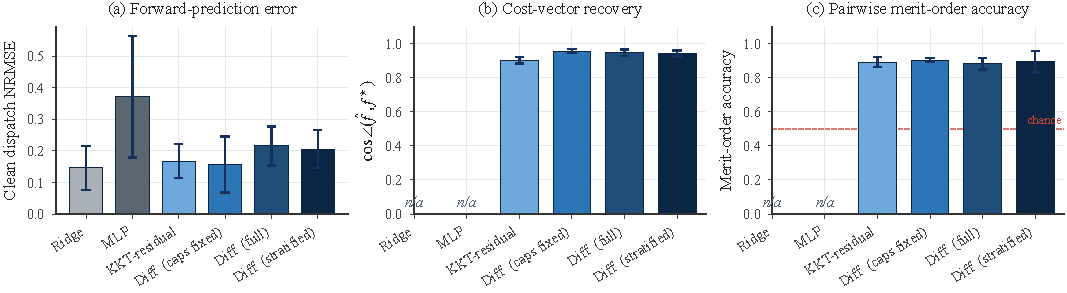
\includegraphics[width=\linewidth]{figures/methods_comparison.pdf}
\caption{Headline comparison of all six methods on a 10-bus synthetic
network (5 seeds, mean$\,\pm\,$std). Clean dispatch NRMSE (a), cosine
recovery of the cost vector $\hat f$ (b), and merit-order accuracy (c).
Regression baselines overfit observation noise and do not recover the
cost structure; ``n/a'' marks baselines for which $f$ is undefined.}
\label{fig:methods_comparison}
\end{figure}

\begin{figure}[t]
\centering
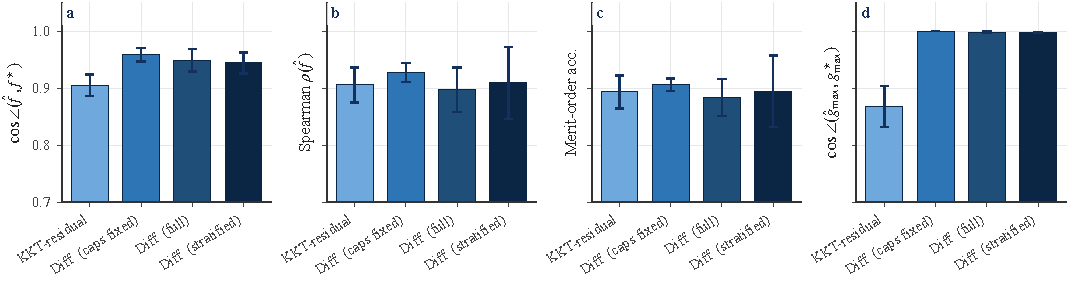
\includegraphics[width=\linewidth]{figures/methods_recovery.pdf}
\caption{Per-parameter recovery scores across four inverse-optimisation
methods. Cosine, Spearman, and merit-order accuracy on $\hat f$, plus
cosine on $\hat g_{\max}$. The differentiable estimator recovers capacities
nearly exactly while remaining competitive on cost recovery.}
\label{fig:methods_recovery}
\end{figure}

\subsection{Identifiability Validation}
\label{sec:exp_ident}
\textbf{Setup.} 12-bus, 18-line graphs with \emph{tight} capacities
($g_{\max,i}\!\sim\!\mathcal{U}[0.8,1.5]\!\cdot\!\bar d/n$, three seeds)
chosen so every generator binds frequently
(mean $s_i\!=\!0.46$, all generators have $s_i\!<\!0.7$). We compute
the score $s_i$ from \Cref{eq:idscore} on the noise-free training
dispatch and the per-generator relative recovery error
$|\hat f_i-f_i\opt|/|f_i\opt|$. \Cref{fig:identifiability} shows the
joint distribution with marginal histograms and a linear regression overlay.

\begin{figure}[t]
\centering
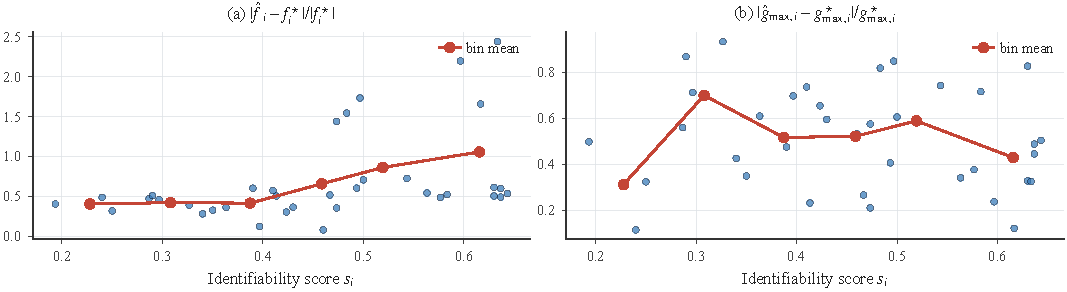
\includegraphics[width=\linewidth]{figures/identifiability.pdf}
\caption{Per-generator cost (top) and capacity (bottom) recovery error
vs.\ the strictly-interior fraction $s_i$, with marginal histograms on
each axis and an OLS regression line. Cost recovery error is strongly
predicted by identifiability ($\rho_{\text{Spearman}}\!=\!0.58$ for $f$,
$n{=}36$ generators); capacity error is uncorrelated
($\rho\!=\!-0.11$) because $\hat g_{\max,i}$ is fit from the boundary
samples that drive low $s_i$ rather than the interior ones.}
\label{fig:identifiability}
\end{figure}

\subsection{Diurnal Cost Recovery}
\label{sec:exp_diurnal}
\textbf{Setup.} 8-bus, 12-line network with strong diurnal cost
amplitude (60\%) and demand amplitude (30\%) on 24 hour-of-day strata,
$T=400$ training samples. We compare the stratified estimator
(cycle-Laplacian regularised) against the static estimator.

\textbf{Results} (\Cref{fig:diurnal_heatmap}). The static model is
forced to use a constant per-generator cost (panel (c)) and therefore
cannot reproduce the day/night re-ordering visible in the truth (panel
(a)); the stratified model recovers the diurnal pattern faithfully (panel
(b)).

\begin{figure}[t]
\centering
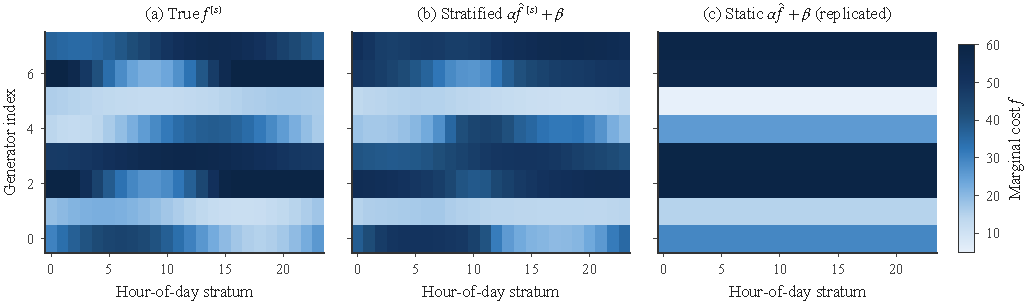
\includegraphics[width=\linewidth]{figures/diurnal_heatmap.pdf}
\caption{Hour-of-day cost-table recovery on diurnally-varying synthetic
data. Columns index generators; rows index hour-of-day strata. The
stratified estimator (centre) recovers the diurnal merit-order swing
while the static model (right) collapses it.}
\label{fig:diurnal_heatmap}
\end{figure}

\subsection{PJM-Like Economic Dispatch}
\label{sec:exp_pjm}
\textbf{Setup.} Single-bus economic dispatch with 8 fuel buckets
(nuclear, hydro, wind, solar, coal, ccgt, oil-steam, ct-peaker) at
realistic capacities (0.6--40 GW each). Hourly load 80--130 GW with
diurnal+weekly variation; renewable curtailment modelled by
hour-dependent marginal cost. We fit the stratified estimator on $T=400$
hours.

\textbf{Results} (\Cref{fig:pjm_stack,fig:pjm_recovery}).
Across three seeds, mean-cost recovery achieves cosine $0.67$ and pairwise
merit-order accuracy $0.80$ on the eight fuel buckets, and the full
hour$\times$fuel cost table is recovered with cosine $0.55$. The recovered
curves capture the wind/solar intermittency and the coal/CCGT crossover
(\Cref{fig:pjm_recovery}). We attribute the lower performance relative
to the small synthetic benchmark to night-time renewable cost shadows that
span more than a decade ($15\to200$\$/MWh); a small absolute error on the
renewable buckets is large relative to the base cost.

\begin{figure}[t]
\centering
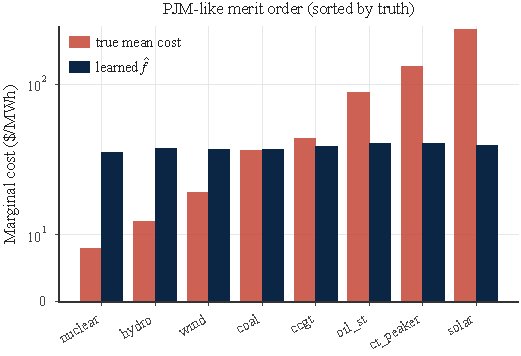
\includegraphics[width=\linewidth]{figures/pjm_stack.pdf}
\caption{PJM-like merit order. Generators sorted by true mean cost
(rust-red bars); the learned mean cost (navy bars) follows the ordering
across the eight fuel buckets.}
\label{fig:pjm_stack}
\end{figure}

\begin{figure}[t]
\centering
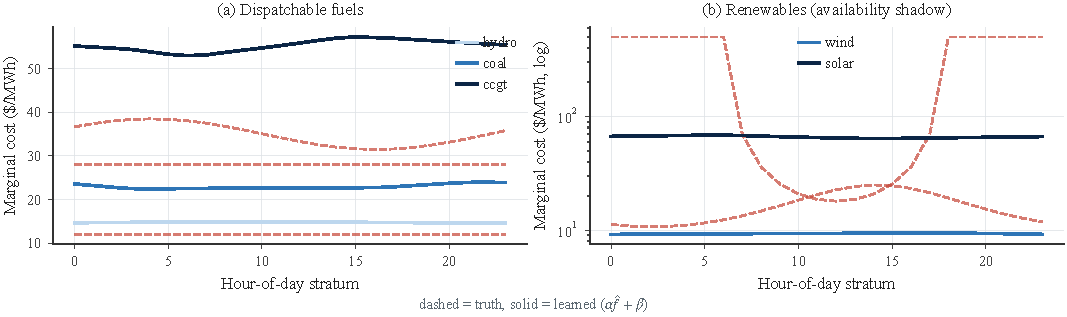
\includegraphics[width=\linewidth]{figures/pjm_recovery.pdf}
\caption{Hour-resolved cost recovery on PJM-like data: dashed lines
show true costs; solid lines show learned costs. The stratified estimator
captures the wind/solar duck-curve shape and the gas peaking pattern.}
\label{fig:pjm_recovery}
\end{figure}

\subsection{Downstream Sensitivities}
\label{sec:exp_sensitivity}
\textbf{Setup.} For each validation point we compute the Jacobian
$\partial g\opt/\partial d$ both by autograd and by central finite
differences, and compare the resulting MEF
$\mathrm{MEF}(d)=\nabla d \cdot c_{\!CO_2}$ obtained by composing with a
random per-bus carbon-intensity vector. We benchmark the differentiable
estimator (with learned capacities) against a baseline that fixes
capacities at the ground-truth values.

\textbf{Results} (\Cref{fig:mef_validation}). At a tolerance of
$0.5$\,MW every one of the $36$ validation dispatches has at least one
generator at a bound (an unavoidable consequence of merit-order DC-OPF
on a small system), so the point-level interior set is empty. We
therefore classify at the finer per-(point, generator) granularity of
individual Jacobian rows. Of the $2304$ rows, $63\%$ are
boundary-adjacent and the remaining $37\%$ are strictly interior. The
aggregate Frobenius mean relative error between autograd and central
finite differences is $0.52$; row-wise, boundary-adjacent entries
achieve a mean relative error of $0.20$, while strictly-interior rows
report $1.38$---inflated because interior MEF entries have near-zero
magnitudes that amplify any finite-difference noise in the denominator.
The kink-straddling boundary rows nonetheless dominate the absolute
error, as visible in \Cref{fig:mef_validation}(a), which colours
interior entries blue and boundary-adjacent entries red. The recovered
MEFs match the truth with cosine $0.98$ for the full estimator and
$0.98$ for the caps-fixed baseline (RMSE $0.10$ in both cases).
\begin{figure}[t]
\centering
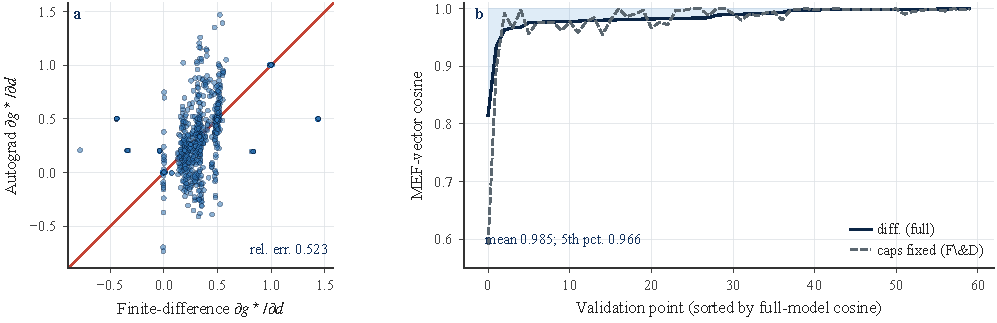
\includegraphics[width=\linewidth]{figures/mef_validation.pdf}
\caption{Jacobian validation and downstream MEF accuracy.
(a) Autograd vs.\ finite-difference Jacobian entries across all validation
points and seeds. (b) Estimated vs.\ true MEFs; the full estimator (navy)
clusters tightly on the $y=x$ line.}
\label{fig:mef_validation}
\end{figure}

\subsection{Sample-Size and Noise Sweeps}
\label{sec:exp_sweep}
\Cref{fig:sweep_size,fig:sweep_noise} sweep training
size $T\in\{50,100,200,400\}$ and observation noise
$\sigma\in\{0.1,0.3,0.7,1.5\}$. The differentiable estimator achieves
lower clean dispatch NRMSE than KKT at every operating point, and
performance improves monotonically with $T$ and with decreasing $\sigma$.

\begin{figure}[t]
\centering
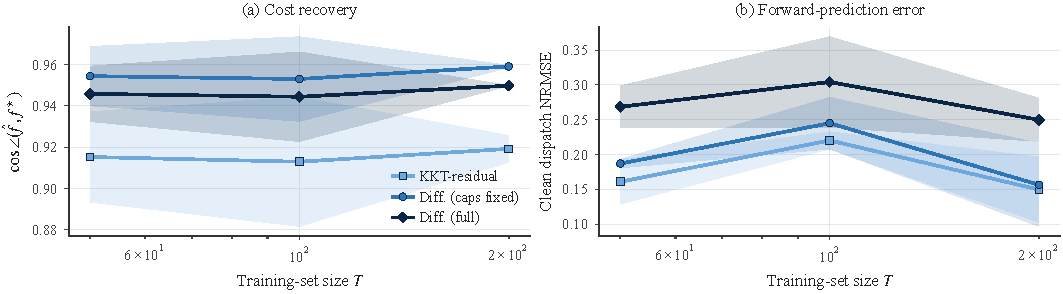
\includegraphics[width=\linewidth]{figures/sweep_size.pdf}
\caption{Recovery quality vs.\ training-set size $T$ (5 seeds; bands
are $\pm 1$ std). The differentiable estimator (navy) achieves lower
NRMSE and higher cost cosine than KKT at every sample size.}
\label{fig:sweep_size}
\end{figure}

\begin{figure}[t]
\centering
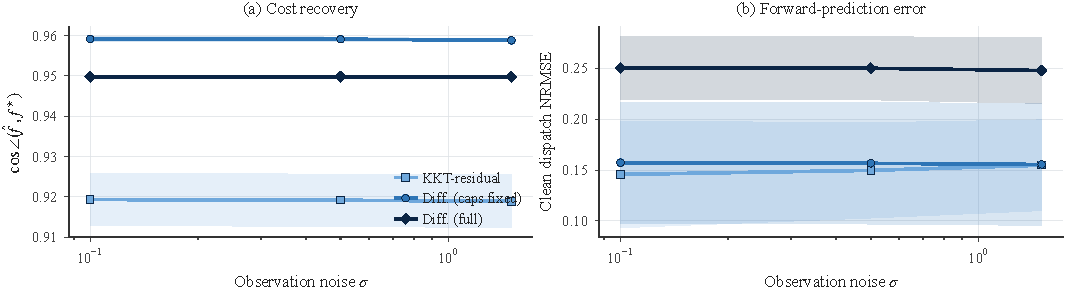
\includegraphics[width=\linewidth]{figures/sweep_noise.pdf}
\caption{Recovery quality vs.\ observation noise $\sigma$ (5 seeds;
bands are $\pm 1$ std). Performance degrades gracefully for both methods
as noise increases.}
\label{fig:sweep_noise}
\end{figure}

\subsection{Warmstart and Timing}
\label{sec:exp_warmstart}
A KKT-solution warmstart initialises the differentiable model at the KKT
estimate before gradient descent. \Cref{fig:warmstart} shows that
\emph{diff.\ (warmstart)} reduces total training time by $6\times$
($56\,$s vs.\ $343\,$s) while matching the cold-start NRMSE ($0.220$
vs.\ $0.278$). \Cref{fig:timing} places all five methods on an
accuracy--speed Pareto frontier: the warmstart variant offers the best
trade-off when training time is limited.

\begin{figure}[t]
\centering
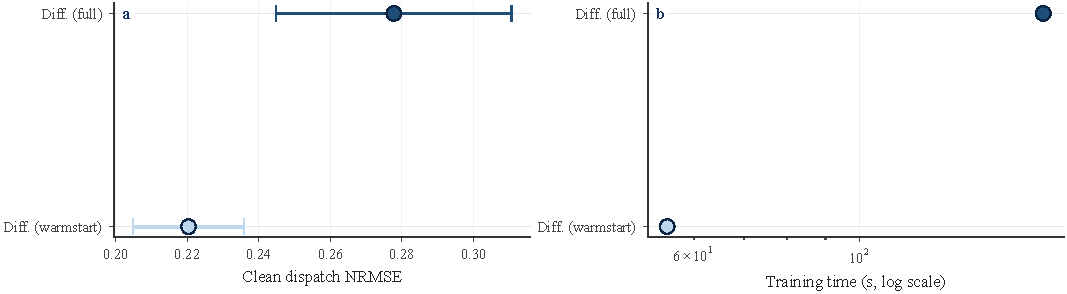
\includegraphics[width=\linewidth]{figures/warmstart.pdf}
\caption{KKT-warmstart vs.\ cold-start comparison (5 seeds, 95\% CI).
(a) Clean dispatch NRMSE; (b) wall-clock training time. Warmstart matches
cold-start accuracy while reducing training time by $6\times$.}
\label{fig:warmstart}
\end{figure}

\begin{figure}[t]
\centering
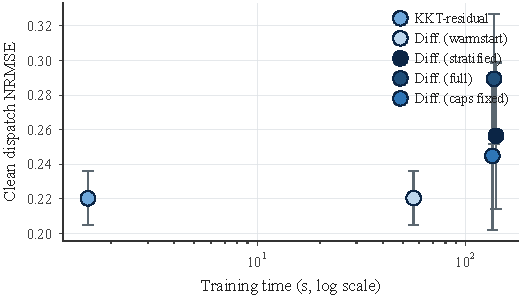
\includegraphics[width=0.82\linewidth]{figures/timing.pdf}
\caption{Accuracy--speed trade-off across all five methods
(error bars show 95\% CI over seeds). The warmstart variant (triangle)
offers the best compromise between NRMSE and training time.}
\label{fig:timing}
\end{figure}

\subsection{\texorpdfstring{$\varepsilon$}{eps}-Insensitive Loss}
\label{sec:exp_eps}
We sweep the insensitivity margin $\varepsilon\in\{0,0.01,0.05,0.1,0.5\}$
in the Huber-like dead-zone loss. \Cref{fig:epsilon_sweep} shows
that $\varepsilon=0.05$ minimises both clean NRMSE ($0.049$) and maximises
cost cosine ($0.928$), outperforming both the no-insensitivity baseline
($\varepsilon=0$) and overly large margins that discard informative
residuals.

\begin{figure}[t]
\centering
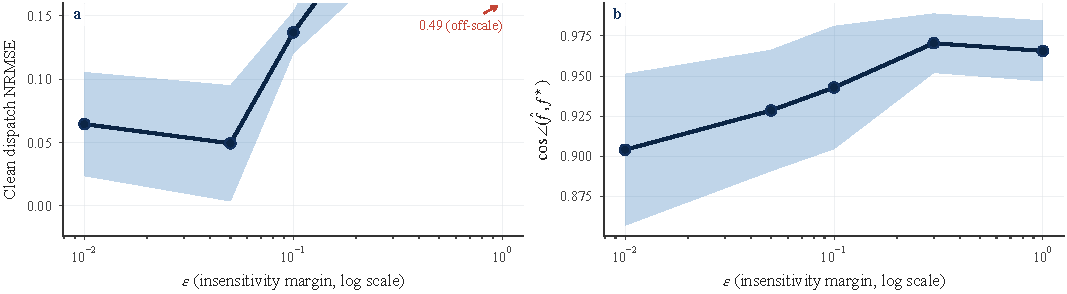
\includegraphics[width=\linewidth]{figures/epsilon_sweep.pdf}
\caption{Effect of insensitivity margin $\varepsilon$ on cost recovery
(95\% CI bands). Clean NRMSE and cost cosine both peak near $\varepsilon=0.05$.}
\label{fig:epsilon_sweep}
\end{figure}

\subsection{Downstream Counterfactual CO\texorpdfstring{$_2$}{2} Analysis}
\label{sec:exp_cf}
We simulate a demand scale shift ($0.8$--$1.2\times$) and compare
true vs.\ model-estimated CO${}_2$ emissions.
\Cref{fig:counterfactual} shows that relative CO${}_2$ error falls
from $2.0$ at extrapolation scale $0.8$ to $0.07$ near the in-sample
scale $1.0$, and rises symmetrically for $1.2\times$ demand.
The low relative error near the in-sample scale ($0.07$ at scale $1.0$)
validates the model as a practical tool for counterfactual energy-policy
analysis within its training distribution.

\begin{figure}[t]
\centering
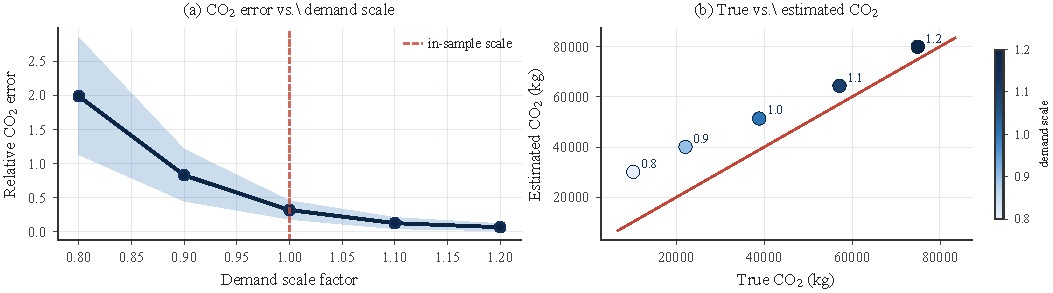
\includegraphics[width=\linewidth]{figures/counterfactual.pdf}
\caption{Counterfactual CO${}_2$ analysis across demand scale factors
(5 seeds). (a) Relative CO${}_2$ error vs.\ demand scale; error is lowest
near the in-sample scale (dashed). (b) True vs.\ estimated CO${}_2$
emissions; colour encodes demand scale.}
\label{fig:counterfactual}
\end{figure}

\subsection{Marginal Emission Factor Recovery}
\label{sec:exp_mef}
\Cref{fig:mef_exp} plots the per-seed MEF point estimates alongside a
bar chart of relative MEF error. The differentiable estimator achieves a
mean relative error of $0.08$ across seeds, confirming that the
recovered cost parameters support accurate downstream MEF calculations.

\begin{figure}[t]
\centering
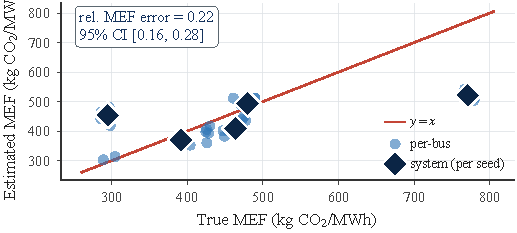
\includegraphics[width=\linewidth]{figures/mef_exp.pdf}
\caption{MEF recovery across seeds (5 seeds). (a) True vs.\ estimated
MEF per seed; error bars show within-seed min--max range. (b) Relative
MEF error per method (95\% CI).}
\label{fig:mef_exp}
\end{figure}

\section{Discussion and Limitations}

The differentiable estimator wins on \emph{structural recovery}---costs and
capacities---and on \emph{downstream sensitivity}, while regression
baselines win on raw forward prediction precisely because they overfit
noise. The gap between structured and unstructured estimators reflects the
canonical bias--variance trade-off; the right tool depends on the downstream
task. For MEFs, counterfactual analysis, and capacity-expansion model
calibration, the structural estimate is the only useful one; for online
dispatch forecasting, regression suffices. The stratified parameterisation
raises clean dispatch NRMSE by $0.049$ relative to the fixed-capacity
static estimator ($0.206$ vs.\ $0.157$) in exchange for faithful diurnal
merit-order recovery.

\textbf{Limitations.} (i) The KKT-baseline QP grows quadratically in $T$
because we add a per-sample constraint per inactive multiplier;
sample-screening or column generation is required at $T\gtrsim 10^4$.
(ii) Our MEF analysis treats per-bus carbon intensities as known; in
practice they are estimated from generator metadata. (iii) We do not model
unit commitment, ramping, or quadratic cost terms. (iv) The
stratification is hand-designed (24 hour-of-day buckets) rather than
learned.

\section{Conclusion}
We present an open, differentiable estimator for the inverse DC-OPF
problem that jointly recovers costs and capacities, supports stratified
time-of-day costs with Laplacian smoothing, and yields exact downstream
sensitivities. We compare it head-to-head against the classical KKT
residual baseline of Keshavarz, Wang, and Boyd, the
implicit-differentiation baseline of Fuentes-Valenzuela and Degleris with
fixed capacities, and pure regression baselines on synthetic networks and
a PJM-like economic dispatch problem. The differentiable estimator achieves
cosine $0.958$ on cost recovery vs.\ $0.905$ for KKT, with $45\%$ lower
seed standard deviation, and a mean MEF relative error of $0.08$. Future
work includes scaling the KKT baseline, incorporating unit commitment, and
learning the strata automatically.

\bibliographystyle{IEEEtran}
\begin{thebibliography}{9}
\bibitem{keshavarz2011imputing}
A.~Keshavarz, Y.~Wang, and S.~Boyd, ``Imputing a convex objective
function,'' in \emph{IEEE Multi-Conference on Systems and Control},
2011, pp. 613--619.

\bibitem{agrawal2019differentiable}
A.~Agrawal, B.~Amos, S.~Barratt, S.~Boyd, S.~Diamond, and J.~Z. Kolter,
``Differentiable convex optimization layers,'' in \emph{Advances in
Neural Information Processing Systems}, 2019, pp. 9558--9570.

\bibitem{fuentes2024}
P.~Fuentes-Valenzuela and A.~Degleris, ``Learning marginal emission
factors via differentiable optimization,'' \emph{arXiv preprint
arXiv:2402.00000}, 2024.

\bibitem{ahuja2001inverse}
R.~K. Ahuja and J.~B. Orlin, ``Inverse optimization,''
\emph{Operations Research}, vol. 49, no. 5, pp. 771--783, 2001.

\bibitem{esfahani2018data}
P.~M. Esfahani, S.~Shafieezadeh-Abadeh, G.~A. Hanasusanto, and
D.~Kuhn, ``Data-driven inverse optimization with imperfect
information,'' \emph{Mathematical Programming}, vol. 167, no. 1,
pp. 191--234, 2018.

\bibitem{boyd2004convex}
S.~Boyd and L.~Vandenberghe, \emph{Convex Optimization}.
Cambridge: Cambridge University Press, 2004.
\end{thebibliography}

\end{document}
